\documentclass[12pt]{article}
\usepackage{preamble}

\pagestyle{fancy}
\fancyhead[LO,LE]{Теория вероятности}
\fancyhead[RO,RE]{Лекции Блаженова А. В.}

\renewcommand{\thesection}{}

\begin{document}

    \tableofcontents
    \clearpage

        % begin probtheory_2024_09_03.tex

    В теории вероятности обычно изучают случайные события

    Обычно наука занимается закономерностями, но так как в случайных экспериментах нет закономерностей, теория
    вероятности занимается поисков закономерности в сериях случайных экспериментах

    Итак, в XVI веке начали с экспериментов бросков монеты:

    \begin{tabular}{ccc}
        число бросков & число гербов & частота \\
        4040 & 2048 & 0.5069 \\
        12000 & 6019 & 0.5016 \\
        24000 & 12012 & 0.5005 \\
    \end{tabular}

    Как можно видеть, частота стремится к 0.5 - появляется статистическая закономерность

    \section{1. Статистическое определение вероятности}

    Пусть проводится $n$ реальных экспериментов, при которых событие $A$ появилось $n_A$ раз

    Отношение $\frac{n_A}{n}$ называется частотой события $A$

    Эксперименты показывают, что при увеличении числа $n$ частота стабилизируется у некоторого числа,
    при котором мы понимаем статистическую вероятность: $P(A) \approx \frac{n_A}{n}$ при $n \to \infty$

    \subsection{Пространство элементарных исходов. Случайные события}

    \Def Пространством элементарных исходов $\Omega$ называется множество, содержащее все возможные исходы
    экспериментов, из которых при испытании происходит ровно один. Элементы этого множества называются
    элементарными исходами и обозначаются $\omega$

    \Def Случайными событиями называется подмножество $A \subset \Omega$. События $A$ наступают, если произошел один из
    элементарных исходов из множества $A$

    \ExN{1} Бросок монеты: $\Omega = \{\text{Г}, \text{Р}\}$, $A = \{\text{Г}\}$ - выпал герб

    \ExN{2} Игральная кость: $\Omega = \{1, 2, 3, 4, 5, 6\}$, $A = \{\text{выпало четное число}\} = \{2, 4, 6\}$

    \ExN{3} Монета бросается дважды.

    a) Учитываем порядок: $\Omega = \{\text{ГГ}, \text{РР}, \text{РГ}, \text{ГР}\}$

    a) Не учитываем порядок: $\Omega = \{\text{ГГ}, \text{РР}, \text{ГР}\}$

    \ExN{4} Кубик дважды: $\Omega = \{\Pair{i, j} \ | \ 1 \leq i, j \leq 6\}$

    $A = \{\text{разность} \ \vdots \ 3\} = \{\Pair{1, 4}; \Pair{4, 1}; \Pair{2, 5}; \Pair{5, 2}; \dots\}$

    \ExN{5} Монета бросается до первого герба: $\Omega = \{\text{Г}, \text{РГ}, \text{РРГ}, \dots\}$ - счетно-бесконечное множество

    \ExN{6} Монета бросается на плоскость: $\Omega = \{\Pair{x, y} \ | \ x, y \in \Real, \Pair{x, y} \text{ - центр монеты}\}$ - несчетное число исходов

    \sebsection{Операции над событиями}

    $\Omega$ - достоверные события (наступают всегда)

    $\emptyset$ - невозможное события (никогда не наступает, так как не содержит ни одного элем. исхода)

    Введем операции:

    \DefN{1} Суммой $A + B$ называется событие, состоящее в том, что произошло события $A$ или событие $B$ (хотя бы одно из них)

    \DefN{2} Произведением $A \cdot B$ называется событие, состоящее в том, что произошло событие $A$ и событие $B$ (оба из них)

    \Notas $A_1 + A_2 + \dots + A_n + \dots$ - произошло хотя бы одно из этих событий

    $A_1 \cdot A_2 \cdot \dots \cdot A_n \cdot \dots$ - произошли все эти события

    \DefN{3} Противоположным $A$ событием называется событие $\overline{A}$, состоящее в том, что событие $A$ не произошло

    \Notas $\overline{A} = A$ % не понял почему

    \DefN{4} Дополнение (разность) $A \setminus B$ называется событие $A \cdot \overline{B}$

    \DefN{5} События $A$ и $B$ называются несовместными, если их произведение - пустое множество
    (не могут произойти одновременно при одной эксперименте)

    \DefN{6} События $A$ влечет события $B$, если $A \subset B$ (если наступает $A$, то наступит $B$)

    \subsection{Вероятность}

    Мы хотим присвоить какую-то числовую характеристику к каждому событию,
    отражающее его частоту наступления: $0 \leq P(A) \leq 1$ - вероятность наступления события $A$

    \mediumvspace

    \textbf{Классическое определение вероятности}

    Пусть пространство случайных событий $\Omega$ содержит конечное число равновозможных исходов,
    тогда применимо классическое определение вероятности

    \Def \fbox{$P(A) = \frac{|A|}{|\Omega|} = \frac{m}{n}$}, где $n$ - число всех возможных исходов, $m$ - число благоприятных исходов

    В частности, если $\Omega = n$ и $A_i$ - элем. исх., то $P(A_i) = \frac{1}{n}$

    Свойства:

    1) $0 \leq P(A) \leq 1$

    2) $P(A) = 1 \quad (m = n)$

    3) $P(\emptyset) = 0 \quad (m = 0)$

    4) Если события $A$ и $B$ несовместны, то $P(A + B) = P(A) + P(B)$

    \mediumvspace

    \textbf{Геометрическое определение вероятности (граф де Бюффон)}

    Пусть $\Omega \subset \Real^n$ - замкнутая ограниченная область

    $\mu(\Omega)$ - мера $\Omega$ в $\Real^n$ (например, длина отрезка, площадь области на плоскости, объем тела в пространстве)

    В эту область наугад бросаем точку. \enquote{Наугад} означает, что вероятность попадания в $A$ зависит только от меры $A$ и не зависит от ее расположения

    В этом случае применимо геометрическое определение вероятности

    $P(A) = \frac{\mu(A)}{\mu(\Omega)}$

    \ExN{1} Монета диаметром в 6 см бросается на пол, вымощенной квадратной плиткой со стороной 20 см, какова вероятность,
    что монета окажется целиком внутри одной плитки

    $\mu(\Omega) = 20^2 = 400$

    $\mu(A) = (20 - 3 - 3)^2 = 196$

    $P(A) = \frac{\mu(A)}{\mu(\Omega)} = \frac{196}{400} = 0.49$

    \ExN{2} Задача Бюффона об игле: пусть пол вымощен ламинатом, $2l$ - ширина доски, на пол бросается игла длины, равной ширине доски,
    найти вероятность того, что игла пересечет стык доски

    \smallvspace

    \begin{minipage}{\linewidth}
        \begin{wrapfigure}{r}{0pt}
            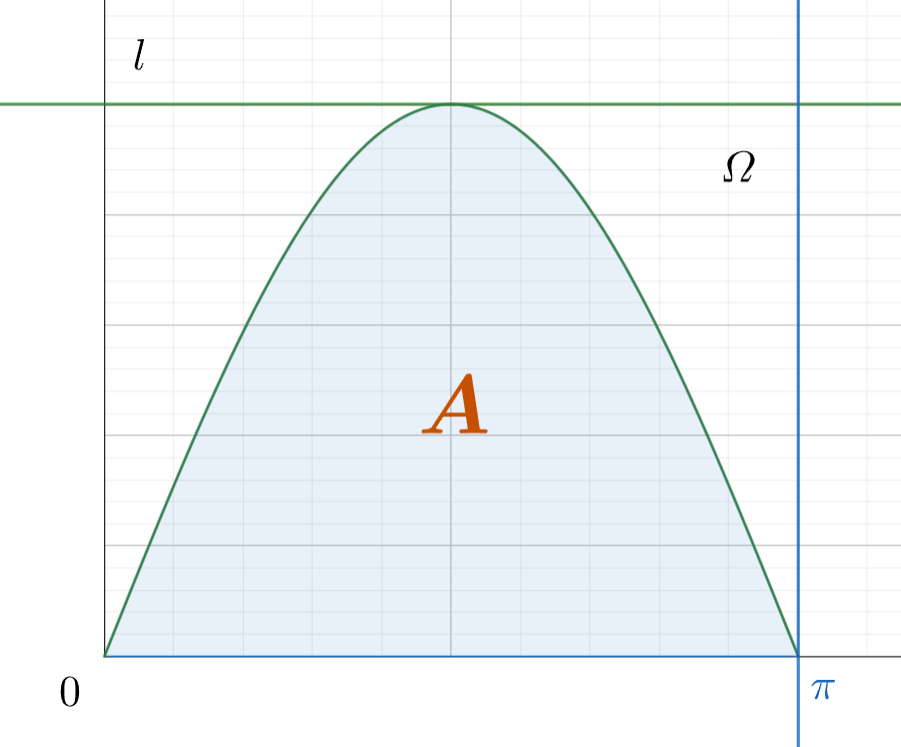
\includegraphics[height=6cm]{probtheory/images/probtheory_2024_09_03_1}
        \end{wrapfigure}

        Определим положение иглы координатами центра и углом, между иглой и стыком доски, причем можно считать, что эти величины независимы

        $\letsymbol x \in [0; 1]$ - расстояние от центра до ближайшего края, $\varphi \in [0; \pi]$ - угол

        $\Omega = [0; 1] \times [0; \pi]$

        Событие $A$ (пересечет стык) наступает, если $x \leq l \sin \varphi$

        $P(A) = \frac{S(A)}{S(\Omega)}$

        $S(\Omega) = \pi l$

        $S(A) = \int_0^\pi l \sin \varphi d\varphi = -l \cos \varphi \Big|_0^\pi = -l (-1 - 1) = 2l$

        $P(A) = \frac{2l}{\pi l} = \frac{2}{\pi}$
    \end{minipage}
    % end probtheory_2024_09_03.tex

    % begin probtheory_2024_09_10.tex

    \subsection{Построение модели случайных явлений}

    \begin{enumerate}
        \item Задаем пространство элементарных исходов $\Omega$

        \item \Defs Система $\mathcal{F}$ подмножеств $\Omega$ называется $\sigma$-алгеброй событий, если:

        1) $\Omega \in \mathcal{F}$;

        2) $A \in \mathcal{F} \Longrightarrow \overline{A} \in \mathcal{F}$;

        3) $A_1, A_2, \dots, A_n, \dots \in \mathcal{F} \Longrightarrow \bigunion_{i = 1}^\infty A_i \in \mathcal{F}$

        \textbf{Свойства}:

        \begin{enumerate}
            \item $\emptyset \in \mathcal{F}$, так как $\Omega \in \mathcal{F} \Longrightarrow \overline{\Omega} = \emptyset \in \mathcal{F}$

            \item $A_1, A_2, \dots \in \mathcal{F} \Longrightarrow \bigcap_{i = 1}^\infty A_i \in \mathcal{F}$

            \begin{tcolorbox}
                $\Box \quad$ $A_1, A_2, \dots \in \mathcal{F} \Longrightarrow
                \overline{A}_1, \overline{A}_2, \dots \in \mathcal{F} \Longrightarrow
                \bigunion_{i = 1}^\infty \overline{A}_i \in \mathcal{F} \Longrightarrow
                \overline{\bigunion_{i = 1}^\infty \overline{A_i}} = \bigcap_{i = 1}^\infty A_i \in \mathcal{F} \quad \Box$
            \end{tcolorbox}

            \item $A, B \in \mathcal{F} \Longrightarrow A \setminus B \in \mathcal{F}$

            \begin{tcolorbox}
                $\Box \quad$ $A, B \in \mathcal{F} \Longrightarrow A, \overline{B} \in \mathcal{F} \Longrightarrow A \setminus B = A \cdot \overline{B} \in \mathcal{F}$ $\quad \Box$
            \end{tcolorbox}

        \end{enumerate}

        \ExNs{1} $\mathcal{F} = \{\emptyset, \Omega\}$

        \ExNs{2} $\mathcal{F} = \{\emptyset, \Omega, A, \overline{A}\}$

        \ExNs{3} \Defs Борелевская $\sigma$-алгебра $\mathcal{B}(\Real)$ - минимальная $\sigma$-алгебра, содержащая все возможные интервалы на прямой

        % на плоскости борелевская сигма-алгебра - прямоугольники

        \item \Defs $\letsymbol\ \Omega$ - пространство элементарных исходов, $\mathcal{F}$ - его $\sigma$-алгебра событий.
        \textit{Вероятностью} на $(\Omega, \mathcal{F})$ называется функция $P: \mathcal{F} \to \Real$ со свойствами:

        \begin{enumerate}
            \item $P(A) \geq 0 \quad \forall A \in \mathcal{F}$ (неотрицательность)

            \item Если $A_1, A_2, \dots, A_n, \dots \in \mathcal{F}$ - несовместное, то $P(\sum_{i = 1}^\infty A_i) = \sum_{i = 1}^\infty P(A_i)$ (свойство счетной аддитивности)

            \item $P(\Omega) = 1$ (условие нормированности)
        \end{enumerate}

    \end{enumerate}

    \Def Из этого тройка $(\Omega, \mathcal{F}, P)$ называется вероятностным пространством

    \subsection{Свойства вероятности}

    \begin{enumerate}

        \item Так как $\emptyset$ и $\Omega$ - несовместные, то $1 = P(\Omega) = P(\Omega + \emptyset) = 1 + P(\emptyset) \Longrightarrow P(\emptyset) = 0$

        \item Формула обратной вероятности: $P(A) = 1 - P(\overline{A})$

        \begin{tcolorbox}
            $\Box \quad$ $A$ и $\overline{A}$ - несовместные и $A + \overline{A} = \Omega \Longrightarrow P(A + \overline{A}) = P(\Omega) = 1$ $\quad \Box$
        \end{tcolorbox}

        \item $P(A) = 1 - P(\overline{A}) \leq 1$

    \end{enumerate}

    \subsection{Аксиома непрерывности}

    Пусть имеется убывающая цепочка событий $A_1 \supset A_2 \supset A_3 \supset \dots \supset A_n \supset \dots$ и $\bigcap_{i = 1}^\infty A_n = \emptyset$

    Тогда $P(A_n) \underset{n \to \infty}{\to} 0$

    При непрерывном изменении области $A \subset \Omega \subset \Real^n$ соответствующая вероятность $P(A)$ также должна изменятся непрерывно

    \Th Аксиома непрерывности следует из аксиомы счетной аддитивности

    \begin{tcolorbox}
        $\Box$

        Ясно, что $A_n = \sum_{i = n}^\infty A_i \overline{A}_{i + 1} + \prod_{i = n}^\infty A_i$

        $\prod_{i = n}^\infty A_i = A_n \cdot \prod_{i = n + 1}^\infty A_i = \prod_{i = 1}^n
        \cdot \prod_{i = n + 1}^\infty A_i = \prod_{i = 1}^\infty = \emptyset \Longrightarrow
        A_n = \sum_{i = n}^\infty A_n \overline{A_{n + 1}}$ и так как эти события несовместны,
        то по свойству счетной аддитивности $P(A_n) = \sum_{i = n}^\infty P(A_i \overline{A_{i + 1}})$ - это остаток (хвост) сходящегося ряда

        $P(A_1) = \sum_{i = 1}^\infty P(A_i \overline{A_{i + 1}}) = \sum_{i = 1}^{n - 1} P(A_i \overline{A_{i + 1}}) + P(A_n)$ и $P(A_n) \underset{n \to \infty}{\to} 0$ по необходимому признаку сходимости

        $\Box$
    \end{tcolorbox}

    \Nota Аксиому счетной аддитивности можно вывести из конечной аддитивности и аксиомы счетной непрерывности

    \textbf{Свойства операций сложения и умножения}

    1. Свойство дистрибутивности: $A \cdot (B + C) = AB + AC$

    2. Формула сложения: если $A$ и $B$ несовместны, то $P(A + B) = P(A) + P(B)$

    3. Формула сложения вероятностей: $P(A + B) = P(A) + P(B) - P(AB)$

    \begin{tcolorbox}
        $\Box$

        $A + B = A\overline{B} + AB + \overline{A}B$ - несовместные события $\Longrightarrow P(A + B) = P(A\overline{B}) + P(AB) + P(\overline{A}B) =
        (P(A\overline{B}) + P(\overline{A}B)) - P(AB) = P(A) + P(B) - P(AB)$

        $\Box$
    \end{tcolorbox}

    \Ex Из колоды в 36 карт достали одну карту. Какова вероятность того, что будет дама или пика

    Пусть Д - дама, П - пика, $P(\text{Д} + \text{П}) = P(\text{Д}) + P(\text{П}) - P(\text{Д}\text{П}) = \frac{4}{36} + \frac{9}{36} - \frac{1}{36} = \frac{1}{3}$

    Формула сложения при $N = 3$: $P(A_1 + A_2 + A_3) = P(A_1) + P(A_2) + P(A_3) - P(A_2 A_3) - P(A_1 A_3) - P(A_1 A_2) + P(A_1 A_2 A_3)$

    Общий случай: $P(A_1 + A_2 + \dots + A_n) =  \sum_{i = 1}^n P(A_i) - \sum_{i < j} P(A_i A_j) + \sum_{i < j < k} P(A_i A_j A_k) + (-1)^{n - 1} \cdot P(A_1 A_2 \dots A_n)$ - формула включения и исключения

    \Ex $n$ писем случайно раскладывается по $n$ конвертам. Найти вероятность того, что хотя бы одно письмо окажется в своем конверте

    $\letsymbol A_i$ - $i$-ое письмо в своем конверте

    $P(A_i) = \frac{1}{n}; P(A_i A_j) = \frac{1}{A^2_n}; P(A_i A_j A_k) = \frac{1}{A^3_n}; P(A_1 A_2 \dots A_n) = \frac{1}{n!}$

    Слагаемых вида $A_i$ - $n$ штук; $A_i A_j$ - $C^2_n$; $A_i A_j A_k$ - $C^3_n$; $A_1 A_2 \dots A_n$ - 1 штука

    $P(A) = P(A_1 + A_2 + \dots + A_n) = n \cdot \frac{1}{n} - C^2_n \frac{1}{A^2_n} + C^3_n \frac{1}{A^3_n} - \dots + (-1)^{n - 1} \frac{1}{n!} = 1 - \frac{1}{2} + \frac{1}{3!} - \dots + (-1)^{n - 1} \frac{1}{n!}$

    Так как $e^{-1} = 1 - 1 + \frac{1}{2} - \frac{1}{3!} + \dots$, то при $n \to \infty \quad P(A) \underset{n \to \infty}{\to} 1 - e^{-1} \approx 0.63$

    Независимые события

    Под независимыми событиями логично подразумевать события, не связанные причинно-следственной связью (то есть когда факт наступления одного не влияет на оценку вероятности другого)

    $\letsymbol |\Omega| = n; |A| = m_1; |B| = m_2$

    Проведем пару независимых испытаний. Тогда получаем пространство элементарных исходов $\Omega \times \Omega$ и $|\Omega \times \Omega| = n^2$

    По основному принципу комбинаторики $|A \cdot B| = m_1 \cdot m_2$

    $P(AB) = \frac{|A \cdot B|}{|\Omega \times \Omega|} = \frac{m_1 m_2}{n^2} = P(A) \cdot P(B)$

    \Def События $A$ и $B$ называются независимыми, если $P(A \cdot B) = P(A) \cdot P(B)$

    \Lab $\letsymbol P(A), P(B) \neq 0$, доказать, что если $A$ и $B$ несовместны, то они зависимы

    Свойство: Если $A$ и $B$ независимы, то независимы $\overline{A}$ и $\overline{B}$, $A$ и $\overline{B}$, $\overline{A}$ и $B$

    Доказательство: $A = A \cdot (B + \overline{B}) = AB + A\overline{B}$ - несовместные события $\Longrightarrow P(A) = P(AB) + P(A\overline{B}) \Longrightarrow P(A\overline{B}) = P(A) - P(AB) =
    P(A) - P(A) \cdot P(B) = P(A) (1 - P(B)) = P(A) P(\overline{B}) \Longrightarrow$ независимы

    \Def События $A_1, A_2, \dots A_n$ - независимы в совокупности, если для любого набора $i_1, i_2, \dots, i_k \ (2 \leq k \leq n)$
    $P(A_{i_1} \cdot A_{i_2} \cdot \dots \cdot A_{i_k}) = P(A_{i_1}) \cdot P(A_{i_2}) \cdot \dots \cdot P(A_{i_k})$

    \Nota Из независимости в совокупности при $k = 2$ получаем попарную независимость. Обратное утверждение неверно

    \Ex (С. Бернштейн)

    Пусть имеется правильный тетраэдр, одна грань окрашена в красный, вторая в синий, третья в зеленый, а четвертая во все эти три цвета.

    Подбросили тетраэдр, $\letsymbol A$ - грань, которая содержит красный цвет, $B$ - синий, $C$ - зеленый.

    $P(A) = P(B) = P(C) = \frac{2}{4} = \frac{1}{2}$

    Так как $P(AB) = P(AC) = P(BC) = \frac{1}{4}$

    $P(AB) = \frac{1}{4} = \frac{1}{2} \cdot \frac{1}{2} = P(A) P(B)$ - попарная независимость

    $P(ABC) = \frac{1}{4} \neq P(A) P(B) P(C)$ - но вот независимость в совокупности не соблюдается

    \Ex (Шевалье де Мере, Паскаль, Ферма, $\approx$ 1650 г.)

    Какова вероятность того, что при 4 бросании кости выпадет одна шестерка

    $A_1$ - при первом броске шестерка, $A_2$ - при втором, $A_3$ - при третьем, $A_4$ - при четвертом

    $B$ - выпала хотя бы одна шестерка при 4 бросках

    $B = A_1 + A_2 + A_3 + A_4$ - совместные события, но независимые

    Найдем обратную вероятность: $\overline{B}$ - ни разу не выпала шестерка

    $\overline{B} = \overline{A_1} \cdot \overline{A_2} \cdot \overline{A_3} \cdot \overline{A_4}$

    $P(\overline{A_1}) = P(\overline{A_2}) = P(\overline{A_3}) = P(\overline{A_4}) = \frac{5}{6}$

    $\overline{B} = P(\overline{A_1}) P(\overline{A_2}) P(\overline{A_3}) P(\overline{A_4}) = \left(\frac{5}{6}\right)^4 \approx 0.482$

    $P(B) = 1 - P(\overline{B}) \approx 0.52$
    % end probtheory_2024_09_10.tex

    % begin probtheory_2024_09_17.tex

    \subsection{Условная вероятность}

    Условная вероятность $P(A|B)$ (или $P_B(A)$) - вероятность события $A$, вычисленная в предположении, что событие $B$ уже произошло

    \Ex Бросается кость один раз, известно, что выпало больше 3 очков. Найти вероятность того, что выпало четное число очков

    \smallvspace

    \begin{minipage}{\linewidth}
        \begin{wrapfigure}{r}{0pt}
            \begin{center}
                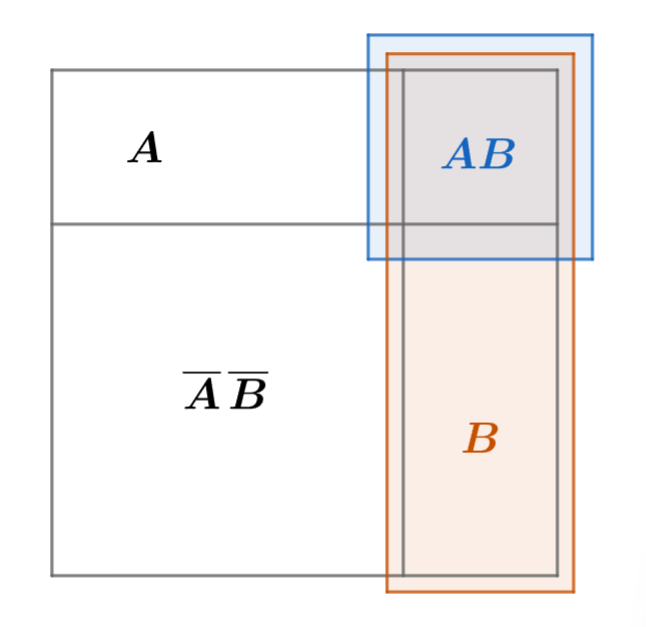
\includegraphics[height=5cm]{probtheory/images/probtheory_2024_09_17_1}
            \end{center}
        \end{wrapfigure}

        $A$ - выпало четное число очков

        $B$ - выпало больше трех очков

        $\Omega = \{1, 2, 3, 4, 5, 6\}; |\Omega| = 6; A = \{2, 4, 6\}; B = \{4, 5, 6\}$

        $P(A|B) = \frac{2}{3} = \frac{\frac{2}{6}}{\frac{3}{6}} = \frac{P(AB)}{P(B)}$


        Интерпретация с помощью геометрической вероятности:

        $P(A|B) = \frac{S_{AB}}{S_B} = \frac{\frac{S_{AB}}{S_\Omega}}{\frac{S_B}{S_\Omega}}$
    \end{minipage}

    \Def Условной вероятностью события $A$ при условии, что имело место событие $B$, называется величина $P(A|B) = \frac{P(AB)}{P(B)}$

    \Ex Известно, что среди населения 1\% воров. В комнате, где находилось 10 гостей, у хозяина пропал кошелек. Какова вероятность того, что произвольный гость является вором.

    $A$ - гость является вором $P(A) = 0.01$

    $B$ - пропал кошелек (хотя бы один вор среди гостей есть)

    $P(A|B) = \frac{P(AB)}{P(B)} = \frac{P(AB)}{1 - P(\overline{B})} = \frac{P(A)}{1 - 0.99^{10}} = \frac{0.01}{1 - 0.99^{10}} = 0.105$

    Формула умножения:

    В качестве следствия условной вероятности получаем:

    $P(A|B) = \frac{P(AB)}{P(B)} \Longrightarrow P(AB) = P(B) \cdot P(A|B) = P(A) \cdot P(B|A)$

    Общий случай:

    $P(A_1 A_2 A_3 \dots A_n) = P(A_1) P(A_2 | A_1) P(P_3 | A_1 A_2) \dots P(A_n | A_1 A_2 \dots A_{n - 1})$

    \begin{tcolorbox}
        $\Box$

        База индукции $P(AB) = P(B) P(A|B)$

        Шаг индукции: пусть верно при $n - 1$:

        $P(A_1 A_2 A_3 \dots A_{n - 1}) = P(A_1) P(A_2 | A_1) P(P_3 | A_1 A_2) \dots P(A_n | A_1 A_2 \dots A_{n - 2})$

        $P(A_1 A_2 A_3 \dots A_n) = P(A_1 A_2 A_3 \dots A_{n - 1}) \cdot P(A_n | A_1 A_2 \dots A_{n - 1}) = \\
        P(A_1) P(A_2 | A_1) P(P_3 | A_1 A_2) \dots P(A_n | A_1 A_2 \dots A_{n - 1})$

        $\Box$
    \end{tcolorbox}


    \Ex Студент выучил 1 билет из $n$, в группе $n$ студентов. Каким по очереди ему нужно зайти, чтобы вероятность сдать экзамен была наибольшей

    Пусть $A_i$ - билет, вытянутый на $i$-ом шаге ($1 \leq i \leq n$)

    $A$ - студент сдал экзамен

    $P(A) = P(\overline{A_1} \cdot \overline{A_2} \cdot \dots \cdot \overline{A_{i - 1}} \cdot A_i) = \frac{n - 1}{n} \cdot \frac{n - 2}{n - 1} \cdot \dots \cdot \frac{n - (i - 1)}{n - (i - 2)} \cdot \frac{1}{n - (i - 1)} = \frac{1}{n}$

    \subsection{Полная группа событий}

    \Def События $H_1, H_2, \dots, H_n, \dots$ образуют полную группу событий, если они попарно несовместны и содержат все возможные элементарные исходы

    $H_i \cap H_j = \emptyset \ \forall i, j \quad\quad\quad \bigunion_{i = 1}^{\infty} H_i = \Omega$

    Следствие: $\sum_{i = 1}^\infty P(H_i) = 1$

    \ThN{Формула полной вероятности} $\letsymbol H_1, H_2, \dots, H_n, \dots$ - полная группа событий. Тогда $P(A) = \sum_{i = 1}^\infty P(H_i) P(A | H_i)$

    \begin{tcolorbox}
        $\Box$

        $P(A) = P(\Omega A) = P((H_1 + H_2 + H_3 + \dots) A) = P(H_1 A + H_2 A + H_3 A + \dots) = [H_i \cdot A \cdot H_j \cdot A = \emptyset \cdot A] = P(H_1 A) + P(H_2 A) + \dots =
        P(H_1) P(A | H_1) + P(H_2) P(A | H_2) + \dots$

        $\Box$
    \end{tcolorbox}

    \ThN{Формула Байеса} $\letsymbol H_1, H_2, \dots, H_n$ - полная группа событий, и известно, что событие $A$ уже произошло

    Тогда $P(H_k | A) = \frac{P(H_k) P(A | H_k)}{\sum_{i = 1}^\infty P(H_i) P(A | H_i)}$

    \begin{tcolorbox}
        $\Box$

        $P(H_k | A) = \frac{P(H_k A)}{P(A)} = \frac{P(H_k) P(A|H_k)}{\sum_{i = 1}^\infty P(H_i) P(A|H_i)}$

        $\Box$
    \end{tcolorbox}

    \ExN{1} В первой коробке 4 белых и 2 черных шара, во второй 1 белый и 2 черных. Из первой коробки во вторую переложили 2 шара, затем из второй коробки достали шар. Какова
    вероятность того, что он оказался белым

    $\letsymbol H_1$ - переложили 2 белых
    $H_2$ - 2 черных

    $H_3$ - разного цвета

    $A$ - из второй коробки достали белый шар

    $P(H_1) = \frac{4}{6} \cdot \frac{3}{5} = \frac{6}{15}$

    $P(H_2) = \frac{2}{6} \cdot \frac{1}{5} = \frac{1}{15}$

    $P(H_3) = \frac{4}{6} \cdot \frac{2}{5} + \frac{2}{6} \cdot \frac{4}{5} = \frac{4}{15} + \frac{4}{15} = \frac{8}{15}$

    $P(A) = P(H_1) \cdot P(A|H_1) + P(H_2) \cdot P(A|H_2) + P(H_3) \cdot P(A|H_3) = \frac{6}{15} \cdot \frac{3}{5} + \frac{1}{15} \cdot \frac{1}{5} + \frac{8}{15} \cdot \frac{2}{5} =
    \frac{18}{75} + \frac{1}{75} + \frac{16}{75} = \frac{35}{75} = \frac{7}{15}$

    \ExN{2} Вероятность попадания первого стрелка в цель $0.9$, а второго $0.3$. Наугад вызванный стрелок попал в цель. Какова вероятность того, что это бы первый стрелок?

    $H_1$ - вызван первый стрелок

    $H_2$ - вызван второй стрелок

    $A$ - стрелок попал

    $P(H_1) = P(H_2) = \frac{1}{2}$

    $P(A|H_1) = 0.9 \quad\quad P(A|H_2) = 0.3$

    $P(H_1 | A) = \frac{P(H_1) P(A|H_1)}{P(H_1) P(A|H_1) + P(H_2) | P(A | H_2)} = \frac{\frac{1}{2} 0.9}{\frac{1}{2} 0.9 + \frac{1}{2} 0.3} = \frac{9}{9 + 3} = 0.75$

    \ExN{3} По статистике раком болеет 1\% населения. Тест дает правильный результат в 99\% случаев. Тест оказался положительный. Найти вероятность того, что человек болен.

    $H_1$ - человек болен

    $H_2$ - человек здоров

    $A$ - анализ положительный

    $P(H_1) = 0.01$

    $P(H_2) = 0.99$

    $P(A|H_1) = 0.99$

    $P(A|H_2) = 0.01$

    $P(H_1 | A) = \frac{P(H_1)P(A | H_1)}{P(H_1) P(A | H_1) + P(H_2) P(A | H_2)} = \frac{0.01 + 0.99}{0.01 \cdot 0.99 + 0.99 \cdot 0.01} = \frac{1}{2} = 0.5$

    Допустим, что второй независимый с первым анализ также оказался положительным. Найти вероятность того, что человек болен.

    $P(H_1) = 0.01 \quad\quad P(H_2) = 0.99$

    $P(AA|H_1) = 0.99^2 \quad\quad P(AA|H_2) = 0.01^2$

    $P(H_1 | AA) = \frac{0.01 + 0.99^2}{0.01 \cdot 0.99^2 + 0.99 \cdot 0.01^2} = \frac{0.99}{0.99 + 0.01} = 0.99$

    Интуитивно вероятность $\frac{1}{2}$ может поддаваться непониманию, однако можно рассуждать так:
    пусть в городе живут 10000 человек, из них 100 болеют, а у 99 из них положительный анализ; у других 9900 положительный анализ всего лишь у 99, отсюда выходит $\frac{1}{2}$

    \ExN{4} В телевизионной студии 3 двери {\Large 🚪🚪🚪}, за одной из них приз {\Large 🚗}.
    Игрок выбрал наугад одну из 3 дверей, после чего ведущий открывает одну из двух оставшихся дверей и показывает, что там приза нет {\Large 🛴}. После чего
    предлагает игроку поменять свой выбор. Стоит ли игроку соглашаться?

    $H_1$ - игрок угадал

    $H_2$ - игрок не угадал

    $A$ - ведущий открыл дверь без приза

    $P(H_1) = \frac{1}{3} \quad\quad P(H_2) = \frac{2}{3}$

    $P(A|H_1) = 1 \quad\quad P(A|H_2) = \frac{1}{2}$

    $P(H_1|A) = \frac{\frac{1}{3} \cdot 1}{\frac{1}{3} \cdot 1 + \frac{1}{3} \cdot \frac{1}{2}} = \frac{1}{2}$

    Но это неправильно, так как действия ведущего неслучайны - он всегда откроет дверь без приза

    В этом случае, если мы гипотетически выберем 300 дверей, в 100 случаях мы отгадаем, ведущий откроет любую дверь без приза;
    но в 200 случаях мы не отгадаем, ведущий откроет вторую дверь без приза, и в этом случае мы сможем поменяться на дверь с призом,
    отсюда шанс $\frac{2}{3}$, если мы поменяем свой выбор \hfill


    \ExN{5} Вероятность того, что в семье с детьми ровно $k$ детей, равна $\frac{1}{2^k}$, $k = 1, 2, \dots$
    Какова вероятность того, что в семье один мальчик, если известно, что нет
    девочки? Рождения мальчиков и девочек равновероятны.


    $H_i$ - в семье $i$ детей ($1 \leq i < \infty$)

    $P(H_i) = \frac{1}{2^i}$

    $A$ - в семье нет девочки

    $P(A|H_1) = \frac{1}{2}$

    $P(A|H_2) = \frac{1}{4}$

    $P(A|H_i) = \frac{1}{2^i}$

    $P(H_1 | A) = \frac{\frac{1}{2} \frac{1}{2}}{\sum_{i = 1}^\infty \frac{1}{2^i} \cdot \frac{1}{2^i}} = \frac{\frac{1}{4}}{\frac{\frac{1}{4}}{1 - \frac{1}{4}}} = \frac{3}{4} = 0.75$
    % end probtheory_2024_09_17.tex



\end{document}

